\documentclass[journal,12pt,twocolumn]{IEEEtran}

\usepackage{setspace}
\usepackage{gensymb}

\singlespacing


\usepackage[cmex10]{amsmath}

\usepackage{amsthm}

\usepackage{mathrsfs}
\usepackage{txfonts}
\usepackage{stfloats}
\usepackage{bm}
\usepackage{cite}
\usepackage{cases}
\usepackage{subfig}

\usepackage{longtable}
\usepackage{multirow}

\usepackage{enumitem}
\usepackage{mathtools}
\usepackage{steinmetz}
\usepackage{tikz}
\usepackage{circuitikz}
\usepackage{verbatim}
\usepackage{tfrupee}
\usepackage[breaklinks=true]{hyperref}
\usepackage{graphicx}
\usepackage{tkz-euclide}
\usepackage{float}

\usetikzlibrary{calc,math}
\usepackage{listings}
    \usepackage{color}                                            %%
    \usepackage{array}                                            %%
    \usepackage{longtable}                                        %%
    \usepackage{calc}                                             %%
    \usepackage{multirow}                                         %%
    \usepackage{hhline}                                           %%
    \usepackage{ifthen}                                           %%
    \usepackage{lscape}     
\usepackage{multicol}
\usepackage{chngcntr}

\DeclareMathOperator*{\Res}{Res}

\renewcommand\thesection{\arabic{section}}
\renewcommand\thesubsection{\thesection.\arabic{subsection}}
\renewcommand\thesubsubsection{\thesubsection.\arabic{subsubsection}}

\renewcommand\thesectiondis{\arabic{section}}
\renewcommand\thesubsectiondis{\thesectiondis.\arabic{subsection}}
\renewcommand\thesubsubsectiondis{\thesubsectiondis.\arabic{subsubsection}}


\hyphenation{op-tical net-works semi-conduc-tor}
\def\inputGnumericTable{}                                 %%

\lstset{
%language=C,
frame=single, 
breaklines=true,
columns=fullflexible
}
\begin{document}


\newtheorem{theorem}{Theorem}[section]
\newtheorem{problem}{Problem}
\newtheorem{proposition}{Proposition}[section]
\newtheorem{lemma}{Lemma}[section]
\newtheorem{corollary}[theorem]{Corollary}
\newtheorem{example}{Example}[section]
\newtheorem{definition}[problem]{Definition}

\newcommand{\BEQA}{\begin{eqnarray}}
\newcommand{\EEQA}{\end{eqnarray}}
\newcommand{\define}{\stackrel{\triangle}{=}}
\bibliographystyle{IEEEtran}
\providecommand{\mbf}{\mathbf}
\providecommand{\pr}[1]{\ensuremath{\Pr\left(#1\right)}}
\providecommand{\qfunc}[1]{\ensuremath{Q\left(#1\right)}}
\providecommand{\sbrak}[1]{\ensuremath{{}\left[#1\right]}}
\providecommand{\lsbrak}[1]{\ensuremath{{}\left[#1\right.}}
\providecommand{\rsbrak}[1]{\ensuremath{{}\left.#1\right]}}
\providecommand{\brak}[1]{\ensuremath{\left(#1\right)}}
\providecommand{\lbrak}[1]{\ensuremath{\left(#1\right.}}
\providecommand{\rbrak}[1]{\ensuremath{\left.#1\right)}}
\providecommand{\cbrak}[1]{\ensuremath{\left\{#1\right\}}}
\providecommand{\lcbrak}[1]{\ensuremath{\left\{#1\right.}}
\providecommand{\rcbrak}[1]{\ensuremath{\left.#1\right\}}}
\theoremstyle{remark}
\newtheorem{rem}{Remark}
\newcommand{\sgn}{\mathop{\mathrm{sgn}}}
\providecommand{\abs}[1]{\lvert#1\vert}
\providecommand{\res}[1]{\Res\displaylimits_{#1}} 
\providecommand{\norm}[1]{\lVert#1\rVert}
%\providecommand{\norm}[1]{\lVert#1\rVert}
\providecommand{\mtx}[1]{\mathbf{#1}}
\providecommand{\mean}[1]{E[ #1 ]}
\providecommand{\fourier}{\overset{\mathcal{F}}{ \rightleftharpoons}}
%\providecommand{\hilbert}{\overset{\mathcal{H}}{ \rightleftharpoons}}
\providecommand{\system}{\overset{\mathcal{H}}{ \longleftrightarrow}}
	%\newcommand{\solution}[2]{\textbf{Solution:}{#1}}
\newcommand{\solution}{\noindent \textbf{Solution: }}
\newcommand{\cosec}{\,\text{cosec}\,}
\providecommand{\dec}[2]{\ensuremath{\overset{#1}{\underset{#2}{\gtrless}}}}
\newcommand{\myvec}[1]{\ensuremath{\begin{pmatrix}#1\end{pmatrix}}}
\newcommand{\mydet}[1]{\ensuremath{\begin{vmatrix}#1\end{vmatrix}}}
\numberwithin{equation}{subsection}
\makeatletter
\@addtoreset{figure}{problem}
\makeatother
\let\StandardTheFigure\thefigure
\let\vec\mathbf
\renewcommand{\thefigure}{\theproblem}
\def\putbox#1#2#3{\makebox[0in][l]{\makebox[#1][l]{}\raisebox{\baselineskip}[0in][0in]{\raisebox{#2}[0in][0in]{#3}}}}
     \def\rightbox#1{\makebox[0in][r]{#1}}
     \def\centbox#1{\makebox[0in]{#1}}
     \def\topbox#1{\raisebox{-\baselineskip}[0in][0in]{#1}}
     \def\midbox#1{\raisebox{-0.5\baselineskip}[0in][0in]{#1}}
\vspace{3cm}
\title{Assignment-4}
\author{Unnati Gupta}
\maketitle
\newpage
\bigskip
\renewcommand{\thefigure}{\theenumi}
\renewcommand{\thetable}{\theenumi}
Download all python codes from 
\begin{lstlisting}
https://github.com/unnatigupta2320/Assignment_4/tree/master/CODES
\end{lstlisting}
%
and latex-tikz codes from 
%
\begin{lstlisting}
https://github.com/unnatigupta2320/Assignment_4
\end{lstlisting}
%
\section{Question No. 2.17}
Find the perpendicular distance of the following lines from the origin and angle between the perpendicular and positive x-axis.
\begin{enumerate}[label=\alph*.]
    \item  $\myvec{1&-\sqrt{3}}\vec{x} =-8$
    \item  $\myvec{0&1}\vec{x} =2$
    \item $\myvec{1&-1}\vec{x} =4$
\end{enumerate}

%
\section{Solution}

\begin{enumerate}
\item For finding the perpendicular distance of lines from origin:
\begin{itemize}
\item Let a point $\vec{A}=\myvec{x\textsubscript{1}\\y\textsubscript{1}}$.
\item The perpendicular distance of a point $\vec{A}$ from a line ax+by+c=0 is given by:-
\begin{align}
d=\frac { \left| a(x\textsubscript{1})+b(y\textsubscript{1})+c \right| }{ \norm{\vec{n}} }
\\
\text{where, } \vec{n}=\myvec{a\\b}
\end{align}
\item If the point is $\vec{O}$= $\myvec{0\\0}$, then
\begin{align}
d &=\frac { \left| a(0)+b(0)+c \right| }{ \norm{\vec{n}}}
\\
d&=\frac { \left| c \right| }{\norm{\vec{n}}}\label{eqA}
\end{align}
\end{itemize}
\item For finding angle between the perpendicular and positive x-axis:-
\begin{itemize}
    \item We have: 
    \begin{align}
    ax+by+c&=0
    \\
    by&=-ax-c
    \\
    y&=\frac{-a}{b}-\frac{c}{b}
    \end{align}
\item So,the slope,m\textsubscript{l} can be written as:
\begin{align}
 m\textsubscript{1}=\frac{-a}{b} \label{eqB}
 \end{align}
\item Let slope of the perpendicular line = m\textsubscript{p},then we know that:
\begin{align}
     m\textsubscript{l}\times m\textsubscript{p}&=-1
     \\
     m\textsubscript{p}&=\frac{-1}{m\textsubscript{l}}
\end{align}
\item Using \eqref{eqB} in above equation we get:
\begin{align}
     m\textsubscript{p}&=\frac{b}{a} \label{eqC}
     \\
  m\textsubscript{p}&=\tan \theta
  \\
  \theta &= \tan^{-1}( m\textsubscript{p})\label{eqD}
\end{align}
\end{itemize}
\item For line, $\myvec{1&-\sqrt{3}}\vec{x}$ =$-8$
\begin{itemize}
\item We have:
\begin{align}
 c\textsubscript{1}=8 , {\vec{n\textsubscript{1}}}=\myvec{1\\-\sqrt{3}}   
\end{align}
\item Using \eqref{eqA} we get:
\begin{align}
d\textsubscript{1}&=\frac { \left| c \right| }{\norm{\vec{n}}}
\\
d\textsubscript{1}&=\frac{8}{\sqrt{1+3}} 
\\
d\textsubscript{1}&=\frac{8}{2}=4\text{ units}
\end{align}
\item Using \eqref{eqC}the slope of the line perpendicular to given line is:
\begin{align}
  m\textsubscript{p1}&=\frac{b}{a}
  \\
  m\textsubscript{p1}&=\frac{-\sqrt{3}}{1}=-\sqrt{3}
\end{align}
 \item Also,Using \eqref{eqD} the angle between Perpendicular and Positive x-axis is:
 \begin{align}
  \theta\textsubscript{1} &= \tan^{-1}( m\textsubscript{2})
  \\
 \theta\textsubscript{1} &= \tan^{-1}(-\sqrt{3}) (\because m\textsubscript{2}=-\sqrt{3})
 \\
 \theta\textsubscript{1} &= -60\degree
\end{align}
\end{itemize}
\item For line, $\myvec{0&1}\vec{x} =2$
\begin{itemize}
\item We have:
\begin{align}
 c\textsubscript{2}=2 ,{\vec{n\textsubscript{2}}}=\myvec{0\\1}   
\end{align}
\item Using \eqref{eqA} we get:
\begin{align}
d\textsubscript{2}&=\frac { \left| c \right| }{\norm{\vec{n}}}
\\
d\textsubscript{2}&=\frac{2}{\sqrt{1}} 
\\
d\textsubscript{2}&=2 \text{ units}
\end{align}
\item Using \eqref{eqC}, the slope of the line perpendicular to given line is:
\begin{align}
  m\textsubscript{p2}=\frac{b}{a}
  \\
\text{But as } a=0 \implies m\textsubscript{p2}=\infty
\end{align}
\item The angle between Perpendicular and Positive x-axis is:
 \begin{align}
 \implies \theta\textsubscript{2} &= \tan^{-1}(\infty)
  \\
 \implies \theta\textsubscript{2} &= 90\degree
\end{align}
\end{itemize}
\item For line,$\myvec{1&-1}\vec{x} =4$
\begin{itemize}
\item We have:
\begin{align}
 c\textsubscript{3}=4 ,{\vec{n}}=\myvec{1\\-1}   
\end{align}
\item Using \eqref{eqA} we get:
\begin{align}
d\textsubscript{3}&=\frac { \left| c \right| }{\norm{\vec{n}}}
\\
d\textsubscript{3}&=\frac{4}{\sqrt{1+1}} 
\\
d\textsubscript{3}&=\frac{4}{\sqrt{2}}
\\
d\textsubscript{3}&=\frac{4}{1.41}
\\
d\textsubscript{3}&=2.828 \text{ units}
\end{align}
\item Using \eqref{eqC} the slope of the line perpendicular to given line is:
\begin{align}
  m\textsubscript{p3}&=\frac{b}{a}
  \\
  m\textsubscript{p3}&=\frac{1}{-1}=-1
\end{align}
 \item Also,Using \eqref{eqD} the angle between perpendicular and positive x-axis is:
 \begin{align}
  \theta\textsubscript{3} &= \tan^{-1}( m\textsubscript{2})
  \\
 \theta\textsubscript{3} &= \tan^{-1}(-1) (\because m\textsubscript{2}=-1)
 \\
 \theta\textsubscript{3} &= -45\degree
\end{align}
\end{itemize}

\item If,
\\
\textbf{d\textsubscript{n}}=Perpendicular distance of line from origin
\\
\\
\textbf{m\textsubscript{pn}}=Slope of the perpendicular to the line 
\\
\\
$\theta\textsubscript{n}$= Angle of perpendicular with positive x-axis.
\\
\item All the given and calculated data can be tabularised in table as \ref{tab:table1}:
\end{enumerate}
\numberwithin{table}{section}
\begin{table}[!ht]
\begin{center}
\begin{tabular}{ | m{2cm} | m{1.2cm}| m{1.2cm} | m{1.2cm} |} 
\hline
 & Line1 & Line2 & Line3 \\
\hline
c\textsubscript{1},c\textsubscript{2},c\textsubscript{3} & 8 & 2 & 4 \\ 
\hline
$\vec{n\textsubscript{1}}$,$\vec{n\textsubscript{2}}$,$\vec{n\textsubscript{3}}$ & $\myvec{1\\-\sqrt{3}}$ & $\myvec{0\\1}$ &$\myvec{1\\-1}$ \\ 
\hline
d\textsubscript{1},d\textsubscript{2},d\textsubscript{3} & 4 & 2 & 2.828 \\ 
\hline
\textbf{m\textsubscript{p1}},\textbf{m\textsubscript{p2}},\textbf{m\textsubscript{p3}} & $-\sqrt{3}$ & $\infty$ & -1 \\ 
\hline
$\theta\textsubscript{1}$,$\theta\textsubscript{2}$,$\theta\textsubscript{3}$& $-60\degree$ & $90\degree$ & $-45\degree$ \\ 
\hline
\end{tabular}
\end{center}
\caption{Data:-Given and Calculated}
\label{tab:table1}
\end{table}
\begin{enumerate}[label=\alph*.]
    \item Plot of Line1 :-

\numberwithin{figure}{section}
\begin{figure}[H]
\centering
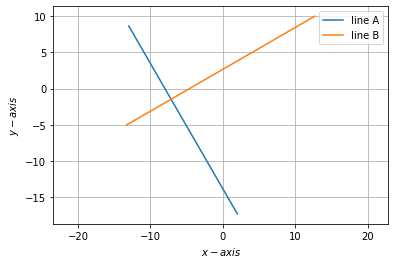
\includegraphics[width=\columnwidth]{Line1 and it's perpendicular.png}
\caption{Line1 and it's perpendicular}
\label{fig:circle}	
\end{figure}


 \item Plot of Line2 :-
\numberwithin{figure}{section}
\begin{figure}[H]
\centering
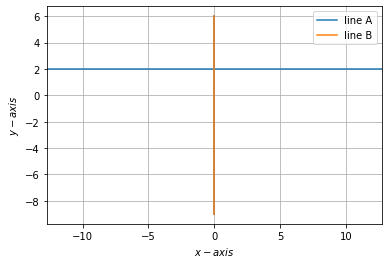
\includegraphics[width=\columnwidth]{Line2 and it's perpendicular.png}
\caption{Line2 and it's perpendicular}
\label{fig:circle}	
\end{figure}
 \item Plot of Line3 :-
\numberwithin{figure}{section}
\begin{figure}[H]
\centering
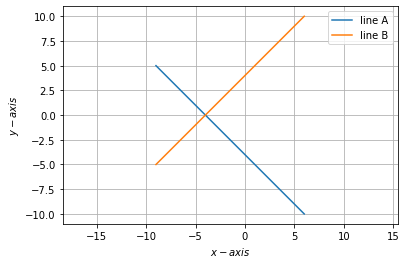
\includegraphics[width=\columnwidth]{Line3 and it's perpendicular.png}
\caption{Line3 and it's perpendicular}
\label{fig:circle}	
\end{figure}

\end{enumerate}
\end{document}
